\section{Equilibrated MD}

Angular analyses were performed to characterize the net molecular orientation of \wat~and \suldiox~molecules. Histograms were created to show the angles $\theta$ and $\phi$ (see figure \ref{fig:water-angles}) relative to a positions from the top surface of the aqueous slab. Both \wat~and \suldiox~orientations are considered for both the neat-\wat~and saturated systems.

\subsection{Water Orientation}

The results of the analyses for \wat~are shown in figure \ref{fig:water-orientation} for both of the surface equilibrated systems. In both systems an orientational preference is found at both the top and bottom slab surfaces. Because the bottom slab is inverted with respect to the top, it is expected that the orientational distributions will reflect the symmetry. The bisector tilt concentrates around $\cos(\theta)=0$ within the first few\angs of the surface, and then the distribution becomes isotropic further into the water bulk. As the tilt nears $\cos(\theta)=0$ the \wat~bisector lies within the plane of the surface indicating a water orientation either flat on the surface, or with some amount of ``twist'' sending the OH bonds in towards, or out of the bulk. The value of $\phi$ determines the ``twist'' in this case. Both systems show a peak in the distributions around $\cos(\phi)=1$ at the water surfaces. This results from an orientation of the water's y-axis (normal to the molecular plane) aligned perpendicular to the plane of the water surface.

Peaks in the distributions of the neat-\wat~system are more clearly pronounced as their intensities are more concentrated and larger than the surrounding area of the profiles. This difference indicates that the transition from the preferred orientation at the water surface has a sharper distinction from the isotropic bulk than in the system with the saturated \suldiox~surface. It appears that the same orientation trend is present in both systems, but the presence of the \suldiox~at the water surface decreases the degree of water orientation at the interface.

\begin{figure}[h!]
	\begin{center}
		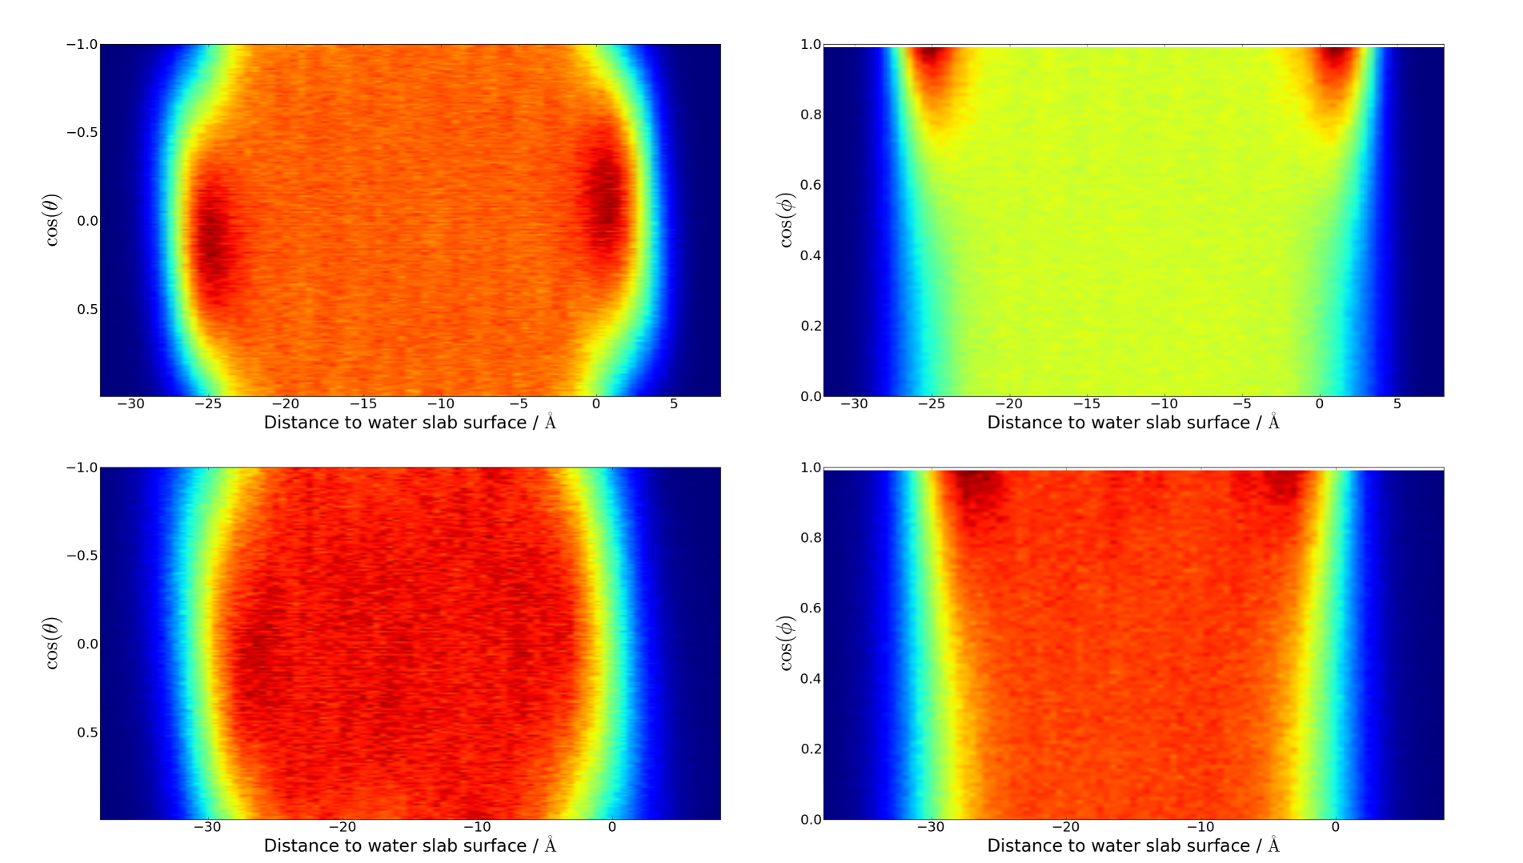
\includegraphics[scale=1.0]{images/waterorientationsmall.png}
		\caption{Molecular orientation histograms of \wat~throughout the surface equilibrated systems. The top surface is located at a distance of 0 with negative positions in the bulk of the slab. The bottom slab surface is approx. 30\angs below the top surface. Shown are the angle distributions for $\theta$ (left column) and $\phi$ (right column) in both the neat-\wat~system (top row) and the saturated system (bottom row).}
		\label{fig:water-orientation}
	\end{center}
\end{figure}

\subsection{\suldiox~Orientation}
